\documentclass{beamer}

\usepackage[utf8]{inputenc}
\usepackage[spanish]{babel}
\usepackage{amsmath}
\usepackage[nosetup]{evan}
%\usetheme{Goddard}
\usetheme{Madrid}
\hypersetup{colorlinks,allcolors=.,urlcolor=magenta}
\usepackage[table]{xcolor} % Para definir colores en tablas
\usepackage{graphicx} % Para redimensionar la tabla
\usepackage{multicol}
\title[IO1]{Investigación de Operaciones I}
\subtitle{Método Simplex}
\author[Ricardo Largaespada]{Ricardo Jesús Largaespada Fernández}
\institute[UNI]{Ingeniería de Sistemas, DACTIC, UNI}
\date{06 de Septiembre, 2024}

\newenvironment<>{varblock}[2][.9\textwidth]{%
  \setlength{\textwidth}{#1}
  \begin{actionenv}#3%
    \def\insertblocktitle{#2}%
    \par%
    \usebeamertemplate{block begin}}
  {\par%
    \usebeamertemplate{block end}%
  \end{actionenv}}
  
\begin{document}

\frame{\titlepage}

\begin{frame}
\frametitle{Agenda}
\tableofcontents
\end{frame}

\section{Representación Tabublar}
\begin{frame}
\frametitle{La representación tabular}
\begin{itemize}
    \item Normalmente omitimos variables al actualizar esos sistemas.
    \item Organizamos los coeficientes en una tabla.
    \begin{itemize}
        \item Como la columna con \(z\) nunca cambia, no la incluimos en la tabla.
    \end{itemize}
    \item Para nuestro ejemplo, el sistema inicial
    \[
    \begin{array}{rcl}
    z - 2x_1 - 3x_2 & = & 0 \\
    x_1 + 2x_2 + x_3 & = & 6 \\
    2x_1 + x_2 + x_4 & = & 8.
    \end{array}
    \]
    \end{itemize}
    \begin{multicols}{2}
    puede expresarse como
    \[
    \begin{array}{ccccc|c}
    -2 & -3 & 0 & 0 & 0 & 0 \\
    \hline
    1 & 2 & 1 & 0 & 1 & 6 \\
    2 & 1 & 0 & 1 & 0 & 8.
    \end{array}
    \]
    \begin{itemize}
    \item Las columnas básicas tienen ceros en la fila 0 y una matriz identidad en las otras filas.
    \item La matriz identidad asocia cada fila con una variable básica.
    \item Un número negativo en la fila 0 de una columna no básica significa que esa variable puede entrar.
    \end{itemize}
    \end{multicols}
\end{frame}

\begin{frame}
\frametitle{Usando tabulares en lugar de sistemas}
    \[
    \begin{array}{rcl}
    z - 2x_1 - 3x_2 & = & 0 \\
    x_1 + 2x_2 + x_3 & = & 6 \\
    2x_1 + x_2 + x_4 & = & 8.
    \end{array}
    \pause
    \quad \Rightarrow \quad
    \begin{array}{ccccc|c}
    -2 & -3 & 0 & 0 & 0 & 0 \\
    \hline
    1 & 2 & 1 & 0 & 1 & 6 \\
    \fbox{2} & 1 & 0 & 1 & 0 & 8.
    \end{array}
    \]
    \pause
    \[
    \begin{array}{rcl}
    z - 2x_2 + x_4 & = & 8 \\
    \frac{3}{2}x_2 + x_3 - \frac{1}{2}x_4 & = & 2 \\
    x_1 + \frac{1}{2}x_2 + \frac{1}{2}x_4 & = & 4.
    \end{array}
    \quad \Rightarrow \quad
    \pause
    \begin{array}{ccccc|c}
    0 & -2 & 0 & 1 & 0 & 8 \\
    \hline
    0 & \fbox{3/2} & 1 & -\frac{1}{2} & 1 & 2 \\
    1 & \frac{1}{2} & 0 & \frac{1}{2} & 0 & 4.
    \end{array}
    \]
    \pause
    \[
    \begin{array}{rcl}
    z + \frac{4}{3}x_3 + \frac{1}{3}x_4 & = & \frac{32}{3} \\
    x_2 + \frac{2}{3}x_3 - \frac{1}{3}x_4 & = & \frac{4}{3} \\
    x_1 - \frac{1}{3}x_3 + \frac{2}{3}x_4 & = & \frac{10}{3}.
    \end{array}
    \quad \Rightarrow \quad
    \pause
    \begin{array}{ccccc|c}
    0 & 0 & \frac{4}{3} & \frac{1}{3} & 0 & \frac{32}{3} \\
    \hline
    0 & 0 & \frac{2}{3} & -\frac{1}{3} & 1 & \frac{4}{3} \\
    1 & 0 & -\frac{1}{3} & \frac{2}{3} & 0 & \frac{10}{3}.
    \end{array}
    \]

\end{frame}

\begin{frame}
\frametitle{El segundo ejemplo}
\begin{itemize}
    \item Consideremos otro ejemplo:
    \[
    \begin{array}{rl}
    \text{max} & x_1 \\
    \text{s.a.} & 2x_1 - x_2 \leq 4 \\
    & 2x_1 + x_2 \leq 8 \\
    & x_2 \leq 3 \\
    & x_i \geq 0 \quad \forall i = 1, 2.
    \end{array}
    \]
    \pause
    \item La forma estándar es
    \[
    \begin{array}{rl}
    \text{max} & x_1 \\
    \text{s.a.} & 2x_1 - x_2 + x_3 = 4 \\
    & 2x_1 + x_2 + x_4 = 8 \\
    & x_2 + x_5 = 3 \\
    & x_i \geq 0 \quad \forall i = 1, \ldots, 5.
    \end{array}
    \]
\end{itemize}
\end{frame}

\begin{frame}
\frametitle{La primera iteración}
\begin{itemize}
    \item Preparamos la tabla inicial. Tenemos \(x^1 = (0, 0, 4, 8, 3)\) y \(z_1 = 0\).
    \[
    \begin{array}{ccccc|c}
    -1 & 0 & 0 & 0 & 0 & 0 \\
    \hline
    2 & -1 & 1 & 0 & 0 & x_3 = 4 \\
    2 & 1 & 0 & 1 & 0 & x_4 = 8 \\
    0 & 1 & 0 & 0 & 1 & x_5 = 3 \\
    \end{array}
    \]
    \pause
    \item Para este problema de \textbf{maximización}, buscamos números \textbf{negativos} en la fila 0. Por lo tanto, \(x_1\) entra.
    \pause
    \begin{itemize}
        \item Esos números en la fila 0 se llaman \textbf{costos reducidos}.
        \pause
        \item La fila 0 es \(z - x_1 = 0\). Aumentar \(x_1\) puede aumentar \(z\).
    \end{itemize}
    \pause
    \item ``Dividir la columna RHS por la columna de entrada'' nos dice que \(x_3\) debe salir (tiene la razón mínima).\footnote{El 0 en la 3ra fila significa que aumentar \(x_1\) no afecta a \(x_5\).}
    \pause
    \begin{itemize}
        \item Esto se llama la \textbf{prueba de la razón}. \textbf{Siempre} buscamos la razón más pequeña.
    \end{itemize}
\end{itemize}
\end{frame}

\begin{frame}
\frametitle{La primera iteración}
\begin{itemize}
    \item \(x_1\) entra y \(x_3\) sale. La siguiente tabla se encuentra pivoteando en 2:
    \[
    \begin{array}{ccccc|c}
    -1 & 0 & 0 & 0 & 0 & 0 \\
    \hline
    2 & -1 & 1 & 0 & 0 & x_3 = 4 \\
    2 & 1 & 0 & 1 & 0  & x_4 = 8 \\
    0 & 1 & 0 & 0 & 1  & x_5 = 3 \\
    \end{array}
    \pause
    \quad \Rightarrow \quad
    \begin{array}{ccccc|c}
    0 & -\frac{1}{2} & \frac{1}{2} & 0 & 0 & 2 \\
    \hline
    1 & -\frac{1}{2} & \frac{1}{2} & 0 & 0 & x_1 = 2 \\
    0 & 2 & -1 & 1 & 0 & x_4 = 4 \\
    0 & 1 & 0 & 0 & 1 & x_5 = 3 \\
    \end{array}
    \]
    \pause
    \item La nueva bfs es \(x^2 = (2, 0, 0, 4, 3)\) con \(z_2 = 2\).
    \pause
    \item ¿Continuar?
    \pause
    \begin{itemize}
        \item Hay un costo reducido negativo en la 2da columna: \(x_2\) entra.
    \end{itemize}
    \pause
    \item Prueba de la razón:
    \pause
    \begin{itemize}
        \item El \(-\frac{1}{2}\) en la 1ra fila muestra que aumentar \(x_2\) hace que \(x_1\) aumente. La fila 1 no participa en la prueba de la razón.
        \pause
        \item Para las filas 2 y 3, la fila 2 gana (con una razón más pequeña).
    \end{itemize}
\end{itemize}
\end{frame}

\begin{frame}
\frametitle{La segunda iteración}
\begin{itemize}
    \item \(x_2\) entra y \(x_4\) sale. Pivotamos en 2.
    \item La segunda iteración es
    \[
    \begin{array}{ccccc|c}
    0 & -\frac{1}{2} & \frac{1}{2} & 0 & 0 & 2 \\
    \hline
    1 & -\frac{1}{2} & \frac{1}{2} & 0 & 0 & x_1 = 2 \\
    0 & 2 & -1 & 1 & 0 & x_4 = 4 \\
    0 & 1 & 0 & 0 & 1 & x_5 = 3 \\
    \end{array}
    \pause
    \quad \Rightarrow \quad
    \begin{array}{ccccc|c}
    0 & 0 & \frac{1}{4} & \frac{1}{4} & 0 & 3 \\
    \hline
    1 & 0 & \frac{1}{4} & \frac{1}{4} & 0 & x_1 = 3 \\
    0 & 1 & -\frac{1}{2} & \frac{1}{2} & 0 & x_2 = 2 \\
    0 & 0 & \frac{1}{2} & -\frac{1}{2} & 1 & x_5 = 1 \\
    \end{array}
    \]
    \pause
    \item La tercera bfs es \(x^3 = (3, 2, 0, 0, 1)\) con \(z_3 = 3\).
    \pause
    \begin{itemize}
        \item Es óptima (¿por qué?).
        \pause
        \item Típicamente escribimos la solución óptima que encontramos como \(x^*\) y el valor objetivo óptimo como \(z^*\).
    \end{itemize}
\end{itemize}
\end{frame}

\begin{frame}
\frametitle{Visualizando el proceso de solución}
\begin{itemize}
    \item Las tres soluciones básicas factibles que obtenemos son:
    \pause
    \begin{itemize}
        \item \(x^1 = (0, 0, 4, 8, 3)\).
        \item \(x^2 = (2, 0, 0, 4, 3)\).
        \item \(x^3 = x^* = (3, 2, 0, 0, 1)\).
    \end{itemize}
    \pause
    \item ¿Encajan con nuestro enfoque gráfico?
\end{itemize}
\pause
\begin{center}
    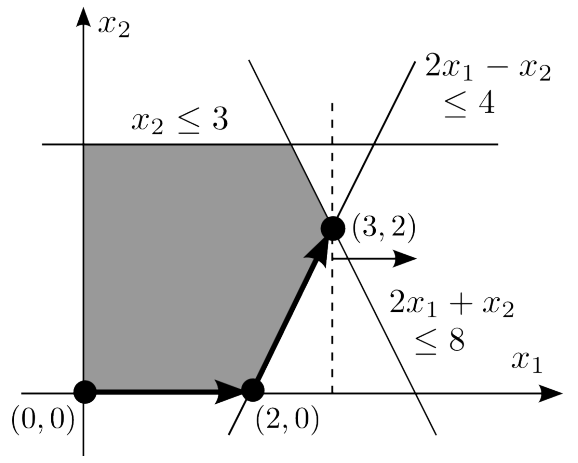
\includegraphics[width=0.6\textwidth]{images/imagen_07.png} % Ruta de la imagen
\end{center}
\end{frame}

\section{No acotación}
\begin{frame}
\frametitle{Identificando la no acotación}
\begin{itemize}
    \item ¿Cuándo es un PL no acotado?
    \item Un PL es no acotado si:
    \begin{itemize}
        \item Existe una dirección de mejora.
        \item A lo largo de esa dirección, podemos movernos indefinidamente.
    \end{itemize}
    \item Cuando ejecutamos el método simplex, esto puede verificarse fácilmente en una tabla simplex.
    \item Consideremos el siguiente ejemplo:
    \[
    \begin{array}{rl}
    \text{max} & x_1 \\
    \text{s.a.} & x_1 - x_2 \leq 1 \\
    & 2x_1 - x_2 \leq 4 \\
    & x_i \geq 0 \quad \forall i = 1, 2.
    \end{array}
    \]
\end{itemize}
\end{frame}

\begin{frame}
\frametitle{PLs no acotados}
\begin{itemize}
    \item La forma estándar es:
    \[
    \begin{array}{rl}
    \text{max} & x_1 \\
    \text{s.a.} & x_1 - x_2 + x_3 = 1 \\
    & 2x_1 - x_2 + x_4 = 4 \\
    & x_i \geq 0 \quad \forall i = 1, \ldots, 4.
    \end{array}
    \]
    \item La primera iteración:
    \[
    \begin{array}{c|cccc|c}
    & x_1 & x_2 & x_3 & x_4 & RHS \\
    \hline
    -1 & 0 & 0 & 0 & 0 & 0 \\
    1 & -1 & 1 & 1 & 0 & x_3 = 1 \\
    2 & -1 & 0 & 1 & 1 & x_4 = 4 \\
    \end{array}
    \quad \Rightarrow \quad
    \begin{array}{c|cccc|c}
    & x_1 & x_2 & x_3 & x_4 & RHS \\
    \hline
    0 & -1 & 1 & 0 & 1 & 1 \\
    1 & -1 & 1 & 1 & 0 & x_1 = 1 \\
    0 & 1 & -2 & 1 & 1 & x_4 = 2 \\
    \end{array}
    \]
\end{itemize}
\end{frame}

\begin{frame}
\frametitle{PLs no acotados}
\begin{itemize}
    \item La segunda iteración:
    \[
    \begin{array}{c|cccc|c}
    & x_1 & x_2 & x_3 & x_4 & RHS \\
    \hline
    0 & -1 & 1 & 0 & 1 & 1 \\
    1 & -1 & 1 & 1 & 0 & x_1 = 1 \\
    0 & 1 & -2 & 1 & 1 & x_4 = 2 \\
    \end{array}
    \quad \Rightarrow \quad
    \begin{array}{c|cccc|c}
    & x_1 & x_2 & x_3 & x_4 & RHS \\
    \hline
    0 & 0 & -1 & 1 & 3 & x_1 = 3 \\
    1 & 0 & -1 & 1 & 1 & x_2 = 2 \\
    0 & 1 & -2 & 1 & 1 & x_4 = 2 \\
    \end{array}
    \]
    \item ¿Cómo podemos realizar la tercera iteración? ¡La prueba de la razón falla!
    \begin{itemize}
        \item Solo las filas con denominadores positivos participan en la prueba de la razón.
        \item ¡Ahora todos los denominadores son no positivos! ¿Qué variable debe salir?
    \end{itemize}
    \item Nadie debería salir: Aumentar \(x_3\) hace que \(x_1\) y \(x_2\) se hagan más grandes.
    \begin{itemize}
        \item Fila 1: \(x_1 - x_3 + x_4 = 3\).
        \item Fila 2: \(x_2 - 2x_3 + x_4 = 2\).
    \end{itemize}
    \item La dirección es entonces una dirección de mejora no acotada.
\end{itemize}
\end{frame}

\begin{frame}
\frametitle{Direcciones de mejora no acotadas}
\begin{itemize}
    \item En \((3,2)\), cuando introducimos \(x_3\), nos movemos a lo largo del borde más a la derecha. 
    \item Geométricamente, ambas restricciones no vinculantes \(x_1 \geq 0\) y \(x_2 \geq 0\) están "detrás de nosotros".
\end{itemize}

\begin{center}
    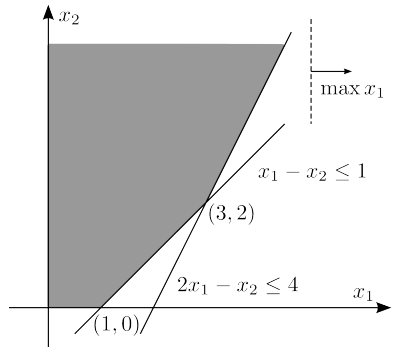
\includegraphics[width=0.6\textwidth]{images/imagen_08.png} % Ruta de la imagen
\end{center}
\end{frame}

\begin{frame}
\frametitle{Detección de PLs no acotados}
\begin{itemize}
    \item Para un PL de minimización, siempre que veamos cualquier columna en cualquier tabla
    \[
    \begin{array}{c|c}
    \overline{c}_j & \\
    \hline
    d_1 & \\
    \vdots & \\
    d_m & \\
    \end{array}
    \]
    tal que \(\overline{c}_j > 0\) y \(d_i \leq 0\) para todo \(i = 1, \ldots, m\), podemos detenernos y concluir que este PL no está acotado.
    \begin{itemize}
        \item \(\overline{c}_j > 0\): Esta es una dirección de mejora.
        \item \(d_i \leq 0\) para todo \(i = 1, \ldots, m\): Esta es una dirección no acotada.
    \end{itemize}
    \item ¿Cuál es la condición de no acotación para un problema de maximización?
\end{itemize}
\end{frame}


\end{document}